\pagestyle{fancy}
\headheight 20pt
\lhead{Ph.D. Thesis --- R. Woods}
\rhead{McMaster - Physics \& Astronomy}
\chead{}
\lfoot{}
\cfoot{\thepage}
\rfoot{}
\renewcommand{\headrulewidth}{0.1pt}
\renewcommand{\footrulewidth}{0.1pt}

\chapter{Radiative Transfer}
\label{chap:radtransfer}

\thispagestyle{fancy}


\section{The Radiative Transfer Problem}
\label{sec:rtformulation}

When considering the transfer of photons, we must consider the scale we are dealing with. At the individual photon level, propagation is described by classical electrodynamics. Once we get to larger scales, however, it is more useful to treat radiation in ``packets'' or as an energy flux.

Consider an infinitesimal patch of area, dA, normal to a direction $\hat{n}$. We consider an infinitesimal solid angle, $d\Omega$, and consider all rays passing through the area and within the solid angle (see figure \ref{fig:intensity}).

\begin{figure}
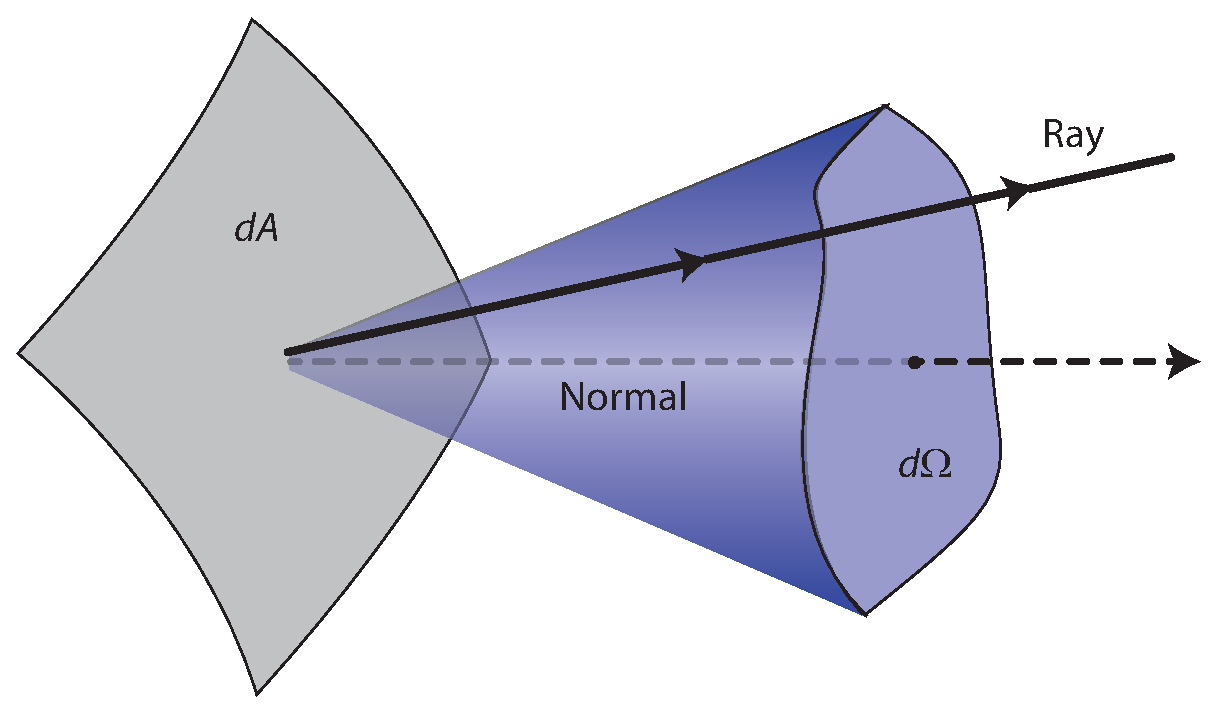
\includegraphics[width=\textwidth]{graphics/intensity.eps}
\caption[A visualization of how intensity is measured.]{The geometry for all rays at a point p through area dA within solid angle $d\Omega$. Figure adapted from \citet{rybickiLightman86}, figure 1.2.}
\label{fig:intensity}
\end{figure}

The energy through this area patch, within the solid angle, in time dt, and within the frequency range $d\nu$ is

\begin{equation}
\label{eq:intensity}
dE = I_{\nu}dA dt d\Omega d\nu,
\end{equation}

\noindent
where $I_{\nu}$ is \emph{specific intensity} (specific because it is within a frequency range; dropping the frequency dependence makes this intensity). Specific intensity has units of energy per unit area per unit time per unit solid angle per unit frequency. It is useful to consider radiation in terms of intensity because it enables a macroscopic description of radiation that includes microscopic effects like scattering and absorption.

We can recover familiar values such as radiative flux, pressure, and density by taking moments of the intensity,

\begin{align}
&E_{\nu} = \int I_{\nu}d\Omega,\nonumber\\
&F_{\nu} = \int I_{\nu}\cos{\theta}d\Omega, \label{eq:moments}\\
&P_{\nu} = \int I_{\nu}\cos^2{\theta}d\Omega,\nonumber
\end{align}

\noindent
where $E_{\nu}$ is the radiation energy density, $F_{\nu}$ is the specific flux (flux at a particular wavelength), and $P_{\nu}$ is the radiation pressure.

Let us now consider the passage of these rays through some matter. If we consider a ray, then energy may be added or removed from this ray due to absorption (removing photons), emission from the matter (adding photons), or scattering (scattering into or out of the ray). Note that throughout the thesis, we consider anything that emits radiation as a source, and any location where radiation is received as a sink. We first consider emission.

We define the specific (monochromatic) emission coefficient, j, as the energy emitted per unit time, per unit solid angle, per unit volume, and per unit frequency,

\begin{equation}
\label{eq:emissioncoef}
dE = j_{\nu} dV dt d\Omega d\nu.
\end{equation}

If we trace along a ray with cross section dA some distance ds, it will cover a cylindrical volume of $dV = dA ds$. Since equation \ref{eq:emissioncoef} and equation \ref{eq:intensity} only differ by a factor of distance (dA compared to dV), we can find the change intensity along the beam due to emission as

\begin{equation}
\label{eq:emissionintensity}
dI = j_{\nu} ds.
\end{equation}

Equation \ref{eq:emissionintensity} describes the amount of intensity added to a ray along some path ds due to spontaneous emission. If emission were the only process to worry about, finding intensity would be a simple matter of integrating the equation.

We next consider absorption. Consider again a ray traveling along a path ds. The amount of intensity lost due to absorption can be defined as

\begin{equation}
\label{eq:absorption}
dI = -\alpha I ds,
\end{equation}

\noindent
where $\alpha$ is called the absorption coefficient and has units of distance$^{-1}$. It can be shown \citep{rybickiLightman86} that $\alpha$ is a function of more commonly known variables,

\begin{equation}
\label{eq:absorptioncoeff}
\alpha = -n \sigma I ds = -\rho \kappa I ds,
\end{equation}

\noindent
where n is the number density of particles, $\sigma$ is the cross section (in units of distance squared) of each absorbing particle, $\rho$ is the mass density, and $\kappa$ is the opacity (in units of distance squared per unit mass). Notice that the only difference between $n \sigma$ and $\rho \kappa$ is the average mass of the absorbing particles. We proceed from here using $\rho$ and $\kappa$, as these values are more directly available in our code.

Finally, we consider scattering. Scattering is a process that both subtracts and adds to the intensity. We can define a specific emission coefficient for scattering by equating the power per unit volume per frequency emitted to the power received,

\begin{equation}
\label{eq:scatteringcoefficient}
j_{s,\nu} = \sigma_{\nu} J_{\nu},
\end{equation}

\noindent
where $\sigma_{\nu}$ is the specific scattering coefficient, and $J_{\nu}$ is the specific mean intensity, defined as

\begin{equation}
\label{eq:meanintensity}
J_{\nu} = \frac{1}{4\pi}\int I_{\nu} d\Omega.
\end{equation}

Before combining all of the processes affecting radiative transfer, it is useful to introduce a variable called the specific \emph{Source Function},

%\begin{align}
%S_{a,\nu} &\equiv \frac{j_{\nu}}{\alpha_{\nu}}, \label{eq:sourcefunction_a}\\
%S_{s,\nu} &\equiv \frac{j_{\nu}}{\alpha_{\nu}}. \label{eq:sourcefunction_s}
%\end{align}

\begin{equation}
\label{eq:sourcefunction}
S_{\nu} \equiv \frac{j_{\nu}}{\alpha_{\nu}}.
\end{equation}

The source function is the ratio of emission to absorption and describes the intensity that an object will tend to. In the case of pure absorption, emission is 0 and so the source function is 0, since the intensity would tend to 0. In the case of pure emission, the source function is infinite and intensity tends to infinity since nothing is removing photons.

We now have the base equations to put together a description of radiative transfer that includes the processes of spontaneous emission, absorption, and scattering. Combining equations \ref{eq:emissionintensity}, \ref{eq:absorption}, \ref{eq:scatteringcoefficient}, \ref{eq:meanintensity}, and \ref{eq:sourcefunction}, we can write

\begin{align}
\label{eq:combinedtransfer}
\frac{dI_{\nu}}{ds} &= (-\alpha_{\nu}I_{\nu} + j_{\nu}) - (\sigma_{\nu}I_{\nu} + j_{s,\nu}) \nonumber\\
 &= -\alpha_{\nu}(I_{\nu} - S_{a,\nu}) - \sigma_{\nu}(I_{\nu} - J_{\nu}) \nonumber\\
 &= -(\alpha_{\nu} + \sigma_{\nu})(I_{\nu}-S_{\nu}),
\end{align}

\noindent
where the combined source function $S_{\nu}$ is defined as

\begin{equation}
\label{eq:combinedsourcefunction}
S_{\nu} \equiv \frac{\alpha_{\nu}S_{a,\nu} + \sigma_{\nu}J_{\nu}}{\alpha_{\nu} + \sigma_{\nu}}.
\end{equation}

The above equation is an integro-differential equation - it is a function of $I_{\nu}$, $\frac{dI_{\nu}}{ds}$, and $\int I_{\nu} d\Omega$. Thus, any equation involving scattering is significantly more difficult to solve. Numerical solutions to integro-differential equations are usually specialized and complex [cite someone], and in the above case, the integral depends on all directions, making it especially costly.

For this reason, scattering is often omitted from radiative transfer solvers due to the very large added computational cost. In this thesis, our solutions do not explicitly account for scattering, though as is discussed in chapter \ref{chap:conclusions}, it is possible to add that functionality.

If scattering is omitted, equation \ref{eq:combinedtransfer} is simplified to a nicer form. We combine equations \ref{eq:emissionintensity}, \ref{eq:absorption}, and \ref{eq:sourcefunction} to obtain

\begin{equation}
\label{eq:transferequation_s}
\frac{dI_{\nu}}{ds} = -\alpha_{\nu}I_{\nu} + j_{\nu}.
\end{equation}

It is now useful to introduce optical depth $\tau_{\nu}$,

\begin{equation}
\label{eq:opticaldepth}
\tau(s) = \int_{s_0}^{s} \alpha_{\nu}(s')ds' = \int_{s_0}^{s} \rho(s') \kappa_{\nu}(s') ds'.
\end{equation}

Optical depth is a unitless value that describes the mean free path of a photon between interactions. The distance needed in the integral to give $\tau_{\nu} = 1$ should correspond to one mean free path given the absorption coefficient $\alpha_{\nu}$. It is useful to rewrite equation \ref{eq:transferequation_s} in terms of $\tau_{\nu}$ and $S_{\nu}$ by simply dividing by $\alpha_{\nu}$

\begin{equation}
\label{eq:transferequation_t}
\frac{dI_{\nu}}{d\tau_{\nu}} = -I_{\nu} + S_{\nu}.
\end{equation}

Equation \ref{eq:transferequation_t} is the transfer equation for radiation as it is most commonly seen. A solution can be obtained by using an integrating factor of $e^{\tau_{\nu}}$, which gives the formal solution to the transfer equation

\begin{equation}
\label{eq:transferequationsolution}
I_{\nu}(\tau_{\nu}) = I_{\nu}(0)e^{-\tau_{\nu}} + \int_0^{\tau_{\nu}} e^{-(\tau_\nu - \tau'_{\nu})} S_{\nu}(\tau'_{\nu})d\tau'_{\nu}.
\end{equation}

Solving the above equation at a point in a simulation would give you a radiation field that accounted for emission and absorption at all other points in the simulation. This would then be repeated at all points for which a radiation field is needed.

It is useful also to consider the case of only absorption. In many astrophysical simulations, only a single or few sources are modeled, and so the emission coefficient is zero at most points. For this reason, it become more efficient to just sum over all sources and treat only absorption. In this case, equation \ref{eq:transferequation_t} simplifies to

\begin{equation}
\label{eq:transferequation_abs}
\frac{dI_{\nu}}{d\tau_{\nu}} = -I_{\nu},
\end{equation}

\noindent
which has the solution

\begin{equation}
\label{eq:absorptionsolution}
I_{\nu}(\tau_{\nu}) = I_{\nu}(0)e^{-\tau_{\nu}}.
\end{equation}

This creates a much simpler (though still quite difficult) problem to solve.

It should now be clear why radiative transfer is a difficult problem; analytically, it involves integrals over source functions that are not necessarily known at all points in space, with both density and opacity varying as a function of position as well. Numerically, we are trying to solve a function of seven variables - three position, two angular, time, and frequency - $I~=~I(x,y,z,\theta,\phi,t,\nu)$.

%\begin{equation}
%\label{eq:rademission}
%I(s) = I(s_0) + \int_{s_0}^{s} j(s') ds'
%\end{equation}
%
%\begin{equation}
%\label{eq:radabsorption}
%I(s) = I(s_0)\exp{\left[-\int_{s_0}^{s} \alpha(s') ds'\right]} = I(s_0)\exp{\left[ -\tau (s) \right]}
%\end{equation}

\section{Current Methods}
\label{sec:currentmethods}

The equations presented in section \ref{sec:rtformulation} are very difficult to solve if approximations are not made. Seven dimensions means that even if each dimension only has a resolution of 100 elements, we must keep track of $10^{14}$ elements, or roughly one petabyte of data if each element is just 10 bytes. In many cases, 100 elements is not nearly fine enough to resolve important features in a dimension, especially in frequency where many sharp features are present. The problem is already numerically impractical from a memory perspective.

As well, the full transfer equation is an integro-differential equation, meaning that common numerical solvers are not useful. Solvers for this type of equation are generally complex and specific purpose, so the actual numerical method side is also difficult.

In order to overcome the above, different approximations to the equation are adopted. Different approximations give rise to different advantages and disadvantages in accuracy and speed and typically apply best to particular regimes.

Current popular strategies include monte-carlo, ray tracing, moment methods, and a variety of others. The following sections will give a brief description of some of the most common and successful techniques as well as common properties of each method.

\subsection{Monte-Carlo Solvers}
\label{sec:montecarlo}

Monte-Carlo (MC) methods are perhaps the most obvious way to solve the radiative transfer problem. The most basic solution follows a photon from emission, through any scattering, absorption, and re-emission, until it leaves the simulation. At any point during the path, random numbers are used to determine whether the photon will be scattered, what direction it will be scattered, whether it will be absorbed, and what wavelength the re-emitted photon(s) will be.

Of course, following individual photons is not practical. Instead, following ``photon packets'' is more useful. Like intensity, packets are typically defined as having a specified energy (in which case, the number of photons can be determined by using $E = h\nu$ \citep{ercolanoEt03,abbottLucy85}.

In order to determine when a photon packet will interact, most codes use one of two methods. The first strategy is to use a probability distribution function (PDF) for optical depth. The PDF takes the form

\begin{equation}
\label{eq:taupdf}
P(l) = \frac{\int_0^{\tau(l)}e^{\tau}d\tau}{\int_0^{\infty}e^{\tau}d\tau} = 1-e^{-\tau},
\end{equation}

\noindent
where P(l) is the probability of an interaction happening at a distance l and $\tau(l)$ is the optical depth corresponding to the interaction. By inverting equation \ref{eq:taupdf}, one can use a random number for P(l) to determine the interaction optical depth (or distance). The photon packet is then assumed to interact at that position, and the process is repeated \citep{harriesHowarth97}.

Another strategy is to simply trace the photon packet from resolution element to resoultion element (cells, particles), and at each point, to use a random number to determine if the photon packet should interact at that cell. This has the advantage that the code does not need to calculate and normalize optical depths \citep{lucy99,ercolanoEt03}.

The above process is repeated until a photon packet leaves the simulation volume, and is performed for many photon packets. Once a large number of photon packets have been sent out, physical quantities must be estimated from observed MC quantities. In this case, a common physical quantity to determine is mean intensity $J$ and the MC quantity is the photon packet. In order to relate the quantities, an \emph{estimator} is needed. An obvious choice (though not necessarily the most optimal \citep{ercolanoEt03}) is to simply use the definition of intensity (equation \ref{eq:intensity}),

\begin{equation}
\label{eq:mcstimator}
\Delta E = I_{\nu}(r,\theta)\Delta A |\cos{\theta}|\Delta \nu \Delta \omega \Delta t,
\end{equation}

\noindent
where $\Delta A$ is the reference surface, $\theta$ is the angle between the photon packet vector and surface normal vector, $\Delta \omega$ is the solid angle, $\Delta \nu$ is the frequency range, and $\Delta t$ is the time interval. By combining with equation \ref{eq:meanintensity}, one can obtain a mean intensity from a sum of photon packets \citep{ercolanoEt03},

\begin{equation}
\label{eq:mcmeanintensity}
J_{\nu}(r) = \frac{1}{4\pi}\frac{\Delta E}{\Delta t} \sum_i^{N_k} \frac{1}{\cos{\theta}}\frac{1}{\Delta A}\frac{1}{\Delta \nu}.
\end{equation}

Once a mean intensity is found at a location, a solution for ionization can be iterated to by integrating out the ionization and heating terms with the mean intensity. Note that it must be iterated since a change in ionization and temperature may imply a change in local absorption properties.

The MC process is very accurate. It can deal with arbitrary spatial distributions, arbitrary scattering functions, polarization, and provides a natural way for ``observing'' a simulated object.

However, MC is \emph{very} computationally costly. Large numbers of photon packets must be sent out and individually tracked in order to get a good estimate of the true mean intensity. Due to the random nature, typically errors only converge as 1/$\sqrt{N_{\gamma}}$, where $\sqrt{N_{\gamma}}$ is the number of photon packets per source. While photons can be added to a packet along its path by gas and dust, new photon packets must be created for all stellar sources to guarantee their emission is added. This means as more sources are added, the computational cost rises linearly.

There is also an indirect cost associated with optical depth. In the case of very optically thick systems, interactions occur far more often between photon packets and the medium, meaning more computation is needed per photon packet. In the case of very optically thin systems, interactions are very rare and very large numbers of photons must be cast to get accurate statistics on heating, ionization, and scattering. 

From a numerical perspective, MC provides poor error control. Higher accuracy requires an increase in the number of photons. However, as was mentioned, this converges very slowly and often still does not guarantee good statistics on rare events such as low probability re-emission or scattering.

For the above reasons, MC radiative transfer is most commonly used as a post-processing technique for creating images of astrophysical objects. For more details on specific codes, please see \citet{dullemond12,cantalupoPorciani11,altayEt08,ercolanoEt03,nenkovaEt99,lucy99,harriesHowarth97}, among many others.

%In monte-carlo methods, a photon is carefully tracked through a domain, following scattering, absorption, and re-emission. See [from steinacker 09] \citet{wolf03,woodEt2004,ercolanoEt2005,jonsson06,pinteEt06}.

%\begin{itemize}
%\item Advantages - can treat complicated spatial distributions, arbitrary scattering functions, and polarization.
%\item Disadvantages - Very high or low optical depths hard (why?), re-emission in all directions over many events hard (why?), no global error control
%\end{itemize}


\subsection{Ray Tracing}
\label{sec:raytracing}

At the most basic level, Ray Tracing is a fairly natural way to go about solving the equations of radiative transfer and is probably the most popular method in astrophysics. Rays are cast from sources and the energy or photons contained in the ray are diminished as it passes through absorbing material \citep{altayTheuns13,rosdahlEt13,altayEt08,rijkhorstEt06,abelWandelt02,razoumovScott99,abelNormanMadau99}. This may sound familiar to section \ref{sec:montecarlo} because many Monte Carlo codes often use a ray tracing approach to follow their photon packets.

Most ray tracing codes tend to start by simplifying the radiative transport equation (\ref{eq:transferequation_s}) by assuming the the emissivity of intervening material is 0. This leads to equation \ref{eq:transferequation_abs}, with the solution of equation \ref{eq:absorptionsolution}.

It remains only for the ray tracer to calculate the optical depth between a source and another point. The simplest strategy to do this is to send rays out that intersect every cell in the simulation, and simply remove photons from the ray as they pass through each cell according to equations \ref{eq:opticaldepth} and \ref{eq:transfersolution_abs}. This process is visualized in figure \ref{fig:raytracing}. In any code where the tracing is done from the source all the way to the sink, it is said to be a ``long characteristics'' code.

\begin{figure}
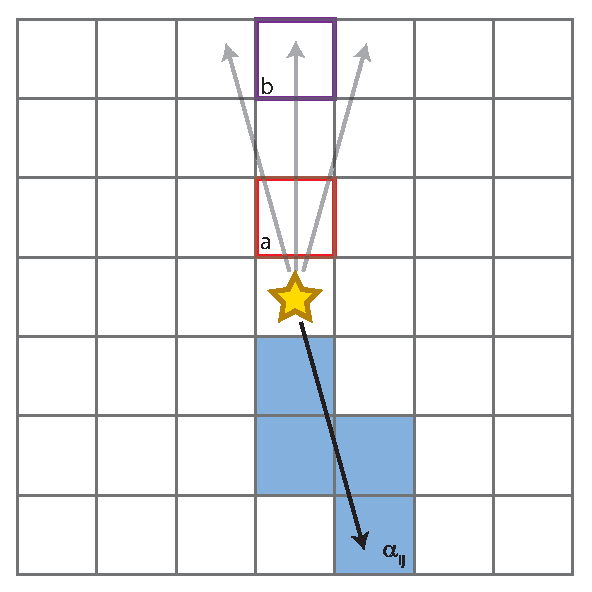
\includegraphics[width=\textwidth]{graphics/ray_flux.eps}
\caption[A visualization of ray tracing.]{Rays being traced through a grid in a simulation. Each ray has an associated energy that is removed from the ray as it traverses through each cell according to the properties of that cell. The blue highlighted cells show an example for one particular ray, where intensity is removed according to the absorption coefficient, $\alpha_{i,j}$, of each cell it passes through. Notice that closer cells, such as cell a, have more rays intersecting them than further cells, such as cell b, meaning redundant work is performed in the close cells.}
\label{fig:raytracing}
\end{figure}

In principle, this process would solve the radiative transfer problem provided enough rays were cast. However, many practical problems arise that require special care. When casting rays, closer cells are intersected by far more rays than far away cells, as can be seen in figure \ref{fig:raytracing}, comparing cells a and b. This means redundant work is performed near the source in order to get sufficient resolution of intensity at large distances. Many codes have created adaptive techniques to reduce the number of rays that are needed. For example, \citet{abelWandelt02} make use of the HEALPIX algorithm \citep{gorskiEt05} to determine rays that create an equal area per ray on a sphere. As the ray moves out and the ratio of the surface area of a cell to the solid angle of a ray decreases, the HEALPIX algorithm is recursively called on a single ray to subdivide it into four smaller rays to better sample further cells. This reduces the number of rays that need to be cast (see figure 2 in \citet{abelWandelt02}).

A more difficult problem that arises is the computational cost associate with more sources. For most ray tracing codes, every additional source requires the whole tracing procedure to be performed again. Due to this limitation of the method, it is not often applied to problems with a large number of sources.

While the above description was based off of the initial assumption that scattering was zero, ray tracing codes do exist that attempt to model scattering in some way. Some authors have chosen to break the field into a direct component (due to ionizing sources) and a diffuse component (due to recombination in gas). The diffuse component can then be tracked and solved separately from the direct component. For example, \citet{razoumovScott99} chooses to use an operator split explicit-implicit scheme to advect the radiation variable along the separate rays. Other authors, e.g. \citet{abelNormanMadau99}, use a similar approach advecting the diffuse radiation, but choose not to keep track of rays at this point.

The scenarios presented up until now have all focused on sending rays out from sources. URCHIN \citep{altayTheuns13} is a ray tracing code that has adopted the opposite strategy of sending rays out from sinks. While this may seem counter-intuitive at first, there are many computational advantages to doing this in particular physical scenarios. \citet{altayTheuns13} designed the algorithm to efficiently model the post-reionization Universe, where radiation is coming from all directions. In this case, tracing rays outward from sinks is guaranteed to find sources of radiation and alleviates any sampling issues associated with choosing sources to start tracing from.

Note that many of the algorithms mentioned above rely on tracing radiation outward along structured data. If the data is unstructured, it is far more difficult to properly estimate what portion of ray segments are affected by absorbing media. As well, it becomes very difficult to ensure that sufficiently many rays are propagated to each resolution element. Unfortunately, this is exactly the scenario that is present in Smoothed Particle Hydrodynamics (SPH) simulations, where resolution elements (particles) are free to move to any location and are thus completely irregular.

A ray tracing strategy to deal with an irregular grid was created by \citet{altayEt08}, called SPHRay. In this scenario, rays are sent out as usual, but a particle's contribution to absorption is determined by an integral along the segment intersecting with the smoothing length of the particle (see figure \ref{fig:particletracing} in chapter \ref{chap:method}). Unfortunately, this method can not guarantee that all sink particles receive a sufficient number of photon packets.

\citet{pawlikSchaye08} have created a ``ray tracing'' scheme called TRAPHIC that is specifically designed to deal with the unstructured nature of SPH simulations and suffers much less from sampling issues. In this ray tracer, radiation is ``traced'' out in cones to neighboring SPH particles (Using cones is significantly different from other ray tracers). However, since particles do not necessary exist in all directions for a given position, virtual particles can be introduced to help propagate radiation through voids without particles. Note that by keeping a fixed solid angle for each particle, a natural adaptivity arises since the same solid angle on a particle further from a source will cover a smaller solid angle with respect to the source. TRAPHIC also introduces a method of merging sources that are close in angle for a receiving gas particles. Merging sources means that the algorithm can handle very large numbers of sources, making it one of the most currently powerful algorithms for cosmological simulations. Any code that propagates from one element to the next rather than from the sink to every element directly is called a ``short characteristics'' code.

The ray tracing method affords many advantages - it can handle arbitrary geometries and gives good error control, meaning very accurate results can be obtained. However, the method is typically limited to simulations that contain small numbers of sources due to poor scaling. As well, at very high optical depths, higher order solvers are often needed and it usually becomes more practical to use a moment method (section \ref{sec:momentmethods}).


%ray tracing need 4piR^2/deltax^2 rays to sample far away cells, gives inner sampling of (r/R)^2, wasteful.
%Ray tracing has the ability to treat arbitrary density distributions, and can use general solvers for ODEs. Fairly accurate and fairly expensive.
%
%\begin{itemize}
%\item Often combined with monte-carlo methods
%\item Provides quite accurate results.
%\item Provides global error control.
%\item Can cause step-size limitations in order to consistently transfer photons.
%\item Becomes impractical at high optical depth and can require complicated solvers.
%\end{itemize}

%razoumovScott99 - account for travel time in similar way I suggested.

\subsection{Moment Methods}
\label{sec:momentmethods}

Moment methods represent a large chunk of astrophysical radiative transfer codes currently available. Very broadly, these methods take moments of the radiative transfer equations and make simplifications to make the equations easier to solve by common techniques.

Specifically, we can start by taking angular moments of the radiative transfer equation (equation \ref{eq:moments}). If this is done in a frame comoving with the radiating fluid and local thermodynamic equilibrium is assumed, we get (to first order in v/c) \citep{mihalasMihalas84}

\begin{align}
&\frac{D\rho}{Dt} + \rho \mathbf{\nabla \cdot v} = 0,\label{eq:rhd1}\\
&\rho \frac{D\mathbf{v}}{Dt} = -\nabla P + \frac{1}{c}\chi_F \mathbf{F},\label{eq:rhd2}\\
&\rho \frac{D}{Dt}\left(\frac{E}{\rho}\right) = -\mathbf{\nabla \cdot F} - \mathbf{\nabla v:P} + 4\pi\kappa_p B - c\kappa_E E,\label{eq:rhd3}\\
&\rho \frac{D}{Dt}\left(\frac{e}{\rho}\right) = -P\mathbf{\nabla \cdot v} - 4\pi \kappa_P B + c\kappa_E E,\label{eq:rhd4}\\
&\frac{\rho}{c^2}\frac{D}{Dt}\left(\frac{\mathbf{F}}{\rho}\right) = -\mathbf{\nabla \cdot P} - \frac{1}{c} \chi_F \mathbf{F}.\label{eq:rhd5}
\end{align}

In the above equations, $D/Dt$ is the convective derivative, defined as $D/Dt \equiv \partial / \partial t + \mathbf{v}\cdot \nabla$. The quantities $\rho$, e, $\mathbf{v}$, and p are the mass density, energy density, velocity, and scalar isotropic pressure, respectively. E, $\mathbf{F}$, and $\mathbf{P}$ are the frequency-integrated radiation energy density, momentum density or flux, and pressure tensor, respectively. E, $\mathbf{F}$, and $\mathbf{P}$ are the zeroth, first, and second order angular moments of intensity (equation \ref{eq:moments}).

%\begin{equation}
%A^n(\mathbf{x},t) = \oint I \cos^{n}{\theta}d\Omega.
%\end{equation}

$\chi_F$ is the flux mean total opacity, $\kappa_P$ is the planck mean absorption opacity, and $\kappa_E$ is the energy mean absorption opacity. $\chi_F$ represents an effective opacity with contributions from absorption and scattering across all wavelengths. $\kappa_P$ is the opacity associated with the emission of thermal radiation. $\kappa_E$ is the opacity associated with absorption. B is the planck function intensity. Finally, c is the speed of light.

Qualitatively, \ref{eq:rhd1} represents mass conservation, \ref{eq:rhd2} is momentum conservation, \ref{eq:rhd3} is radiation energy conservation, \ref{eq:rhd4} is gas internal energy conservation, and \ref{eq:rhd5} describes the evolution of flux.
%\subsubsection{Flux Limited Diffusion}

%add whitehouse & bate
One popular moment method is Flux Limited Diffusion (FLD) \citep{almeWilson74,levermorePomraning81,pomraning83,meliaZylstra91,anileRomano92}. In FLD, the assumption is made that intensity is a slowly varying function of space and time. This is certainly true in the limit of very high or very low optical depth. It is the intermediate region ($\tau \approx 1$) where this assumption may not be true. This assumption allows the radiative flux to be written in the form of Fick's Law of diffusion \citep{levermorePomraning81},

\begin{equation}
\label{eq:fluxfdiffusion}
\mathbf{F} = -D\nabla E,
\end{equation}

\noindent
where D is the diffusion coefficient, given by

\begin{equation}
\label{eq:diffusioncoeff}
D = \frac{c\lambda}{\chi},
\end{equation}

\noindent
where $\lambda$ is a dimensionless function of energy called the flux limiter.

In order to solve equations \ref{eq:rhd1}-\ref{eq:rhd5}, the system must be closed by relating the moments of radiation. A common choice is the Eddington Approximation, which assumes the field is isotropic, which implies that

\begin{equation}
\label{eq:eddingtonapprox}
\mathbf{P} = \frac{1}{3}E.
\end{equation}

Using this approximation, equation \ref{eq:rhd5} becomes

\begin{equation}
\label{eq:eddingtonrhd}
\mathbf{F} = -\frac{c}{3\chi}\nabla E,
\end{equation}

\noindent
which is correct in the optically thick limit, but gives an infinite speed of light in optically thin regions. Thus, the flux limiter in equation \ref{eq:diffusioncoeff} functions to allow the Eddington Approximation to be made by by limiting the radiation propagation speed in the optically thin regime.

By combining equations \ref{eq:fluxfdiffusion} and a relationship between moments of intensity, equations \ref{eq:rhd1}-\ref{eq:rhd4} can be solved numerically \citep{turnerStone01}.

Other common moment methods follow a similar path, but use different assumptions for the closure relation. Another popular choice is called the ``M1 closure relation'' \citep{rosdahlTeyssier15, skinnerOstriker13,aubertTeyssier08,auditGonzalez06,levermore84}. This assumes that intensity is rotationally invariant about the direction of radiative flux, rather than fully isotropic. This assumption allows better results in particular scenarios (e.g. shadowing behind dense objects \citep{skinnerOstriker13}) and a more efficient numerical solution \citep{gonzalezEt07,aubertTeyssier08}. However, its applications are limited as it cannot deal with complex radiation fields from distributed sources.

%add stone et al 92
The majority of moment methods tend to have a difficult time dealing with complex source distributions because they adopt a closure relation that only accounts for local characteristics of the radiation field. One moment code (among others) that has managed to get around this is OTVET \citep{gnedinAbel01}. OTVET explicitly constructs the radiation pressure tensor ($\mathbf{P}$ in equations \ref{eq:rhd1}-\ref{eq:rhd5}) from the source distribution in the simulation, removing the need to assume a relationship between moments. This enables a combination of contributions to the intensity from all sources.

Overall, moment methods provide a useful and efficient way to solve problems that consist of high optical depth, where the radiation field is highly isotropic, or low optical depth with simple source distributions.

However, the method has its limitations. Moment methods tend to be very diffusive, which is not always desired. Different closure relations can change the nature of the diffusion, but all moment methods have it in some capacity. Time step limitations are another consideration. The diffusion equation implies a time step that scales as $\Delta x^2/v$, where v is a characteristic speed. In the case of FLD, this is either the speed of light or the ionization propagation speed. As resolution resolution improves, $\Delta x$ decreases on top of an already very large characteristic speed, which means the stable time step becomes prohibitively small. Often in order to ensure reasonable solutions, an implicit method is required, which can require many iterations to converge.

Overall, while moment methods are still more appropriate for large optical depths, the computational cost can still easily become prohibitive (e.g. \citet{bate12} required 34 months of computer time for a simulation of 10$^7$ particles, a fairly average resolution).

\subsection{Other Methods}
\label{sec:othermethods}

Sections \ref{sec:montecarlo}-\ref{sec:momentmethods} cover some of the most common radiative transfer methods currently used in astrophysics. However, it is worth mentioning a few other methods that aren't as easily grouped into the above categories.

In order to overcome some of the shortcomings of moment methods and ray tracing methods, some authors have created hybrid codes that use both methods in different regimes in the simulation. \citet{kuiperEt10} has created one such scheme. The basic idea is to attempt to use each method in the regime where it's most advantageous to save on computation and improve accuracy. In the case of \citet{kuiperEt10}, the algorithm is designed to approach the problem of massive star formation. It uses a first order ray tracer to transfer stellar photons at higher frequencies to the gas. A secondary moment method (FLD) then diffuses the photons through high density gas. This is meant to efficiently model transfer of high frequency photons from a massive star and reprocessing of those photons to lower frequency emission.

The method avoids the difficulties that ray tracing can have in high optical depth regions and benefits from the speed and accuracy of FLD in appropriate physical regions. While the hybrid code of \citet{kuiperEt10} was specialized to do simulations of a single massive star, the code has since been extended to work on an arbitrary number of sources \citep{klassenEt2014}.

Another strategy is to make use of the Fast Fourier Transform (FFT) techniques. \citet{cen02} makes use of the property that if the sum of a quantity over a volume can be written in the standard convolution form, than it can be solved using an FFT. By re-writing equations \ref{eq:} and \ref{eq:} in this form, one can solve the equations in $N\log(N)$ time for each direction. Using trees to discretize the angles, you end up with roughly $\log(N)$ angles to solve for, and so the solution scales as $N\log^2(N)$.

Finally, \citet{clarkEt12} have created an algorithm most similar to ray tracers, but whose purpose is to calculate column depths for exterior sources. The basic idea is to map the simulation volume onto a sphere that has been divided into equal area segments by the HEALPIX algorithm \citep{gorskiEt05}. By performing this action during the tree walk, columns can be calculated to any point within the simulation at a cost of $N\log(N)$. However, since this algorithm only calculates column depth as a function of $\theta, \phi$ for each particle, it is limited to cases in which sources are located outside of all absorbing material. As well, since each particle must retain a full optical depth map of the sky, memory costs become very high.

%Grid methods, statistic approach (MC?), fourier transforms (cen), hybrid methods (rijkhorst, mikhail), treeCOL, TRAPHIC.

%\subsection{Grid-Based Methods}
%\label{sec:gridmethods}
%
%Can use simple solvers (finite differencing or short characteristics) and gives good error control.
%
%\begin{itemize}
%\item Grid must be adaptable to be practical, though good refinement criteria is unclear
%\item Interpolation between grids can be costly and give interpolation errors.
%\item Numerical diffusion typically not taken into account.
%\end{itemize}

\section{Summary of Methods}
\label{sec:summaryofmethods}

Section \ref{sec:currentmethods} gave an overview of some of the most common methods currently used in astrophysics, so we are now well posed to assess the field of computational radiative transfer.

In order to solve the equations of radiative transfer, codes must make certain approximations. In most codes, authors typically start by dropping scattering. Moment methods typically make a further assumption about the relationship between the moments of radiation, with the most common being the Eddington Approximation (equation \ref{eq:eddingtonapprox}), or the assumption of radiation isotropy.

The above assumptions are still often not sufficient to make the problem computationally viable. Ray tracing has needed to make algorithm-specific improvements to become more computationally efficient. Making rays adaptive as they get further from the source reduces redundant work near the source, and in some scenarios, tracing the rays backwards from the sinks can provide another efficiency boost. Some codes, both ray tracing and moment methods, have also made the improvement of merging sources, which can reduce the number of sources to do calculations for from N to as few as $\log(N)$.

Very roughly, the current code base occupies particular niches in computational radiative transfer. Monte Carlo codes are typically the most accurate, but also the most computationally expensive. For this reason, they are usually limited to post processing and image creation in simulations. Ray tracers are the most popular, and offer very good accuracy, but typically scale quite poorly with the number of sources, and so are usually limited to simulations containing small numbers of sources. Moment codes are a step up in computational speed, but are usually only appropriate in simulations that have high optical depth where the assumption of radiation isotropy is appropriate. Otherwise, unwanted diffusion in the radiation field can give large errors. Despite the simplifying assumptions, many moment codes are still the dominant computational cost in simulations due to time step considerations and solver behavior.

Currently, there is a gap in the market for solvers that can deal with large numbers of sources over a range of optical depths without any diffusive assumptions. OTVET \citep{gnedinAbel01} is close to this regime, and perhaps the most widely recognized tool for cosmological simulations at the time, but is still a diffusive code. TRAPHIC is currently the only code that satisfies the above criteria, and has recently started to take impressive steps forward on the computational cosmology front \citep{jeonEt15, jeonEt14b, jeonEt14a, rahmatiEt13b, rahmatiEt13a,jeonEt12}. TRAPHIC is SPH-specific, and so the algorithm is limited in this way. However, it is probably the most appropriate tool at the time for cosmological radiative transfer.

%\citep{pawlikEt15,jeonEt15,jeonEt14b,jeonEt14a,pawlikEt14,rahmatiEt13b,rahmatiEt13a,jeonEt12}

The goal of this thesis is to present a new algorithm for solving radiative transfer that is capable of dealing with large numbers of sources, non-diffusive, at a similar computational cost to gravity. In order to achieve these goals, we do not stress achieving exact solutions, but aim for correct qualitative behavior and correct equilibrium solutions.

%The current set of computational methods can be classified as follows:
%
%\begin{itemize}
%\item Very accurate, expensive methods - monte carlo, ray tracing
%\item Methods accurate in specific scenarios, e.g. FLD for optically thick, ``str\"omgren method'' from Dale
%\item \emph{Very} rough approximations, e.g. method that only looks at absorption near sink and source.
%\end{itemize}
%
%As will be seen, there is currently an opening in the market for something in the middle - Decent accuracy at a low cost.

